\section{\faWrench\ Retrieval Augmented Generation\\{\small Parte 2 - Approccio Document to vector store}} % (fold)
\label{sec:spring-ai-rag-part-2}
%
\begin{frame}[t,fragile] \frametitle{Progetto Spring AI}
    \framesubtitle{Applicazione e passaggi}
    {\small
    \begin{itemize}[leftmargin=10pt,align=right]
        \onslide<1->\item[\alert{\faArrowCircleRight}] \textit{Chatbot} Ollama-HR-Venis-ITA e Gemini-HR-Venis-ENG
        \onslide<2->\item[\alert{\faExclamationTriangle}] Approccio classico (informazione testuale estratta tramite documento)
        \begin{itemize}[leftmargin=10pt,align=right]
            \onslide<3->\item[\alertedcircled{1}] Modifica dipendenze di progetto
            \onslide<4->\item[\alertedcircled{2}] Modifica configurazione e profilo applicativo
            \onslide<5->\item[\alertedcircled{3}] Creazione \textit{prompt templates} per strategia RAG
            \onslide<6->\item[\alertedcircled{4}] Creazione \textit{component} per popolamento \textit{vector store} (dati Venis-HR)
            \onslide<7->\item[\alertedcircled{5}] \textit{Test} delle funzionalità con Postman/Insomnia
        \end{itemize}
    \end{itemize}
    }
\end{frame}
%
\begin{frame}[t,fragile] \frametitle{Progetto Spring AI}
    \framesubtitle{RAG}
        \begin{block}{Dipendenze di sistema aggiuntive}
			{\tiny\inputminted{xml}{code/pom.xml}}
    	\end{block}
\end{frame}
%
\begin{frame}[t,fragile] \frametitle{Progetto Spring AI}
    \framesubtitle{RAG}
        \begin{block}{Configurazione applicativo}
			{\tiny\inputminted{yaml}{code/application.yml}}
    	\end{block}
\end{frame}
%
\begin{frame}[t,fragile] \frametitle{Progetto Spring AI}
    \framesubtitle{RAG - Profilo applicativo}
        \begin{block}{File \texttt{application-rag-document-to-vector-store.yml}}
			{\tiny\inputminted{yaml}{code/application-rag-document-to-vector-store.yml}}
    	\end{block}
\end{frame}
%
\begin{frame}[t,fragile] \frametitle{Progetto Spring AI}
    \framesubtitle{Prompt per strategia RAG - Italiano}
        \begin{block}{\textit{File} \texttt{templates/get-rag-hr-data-system-ita-prompt.st}}
			{\scriptsize\inputminted{text}{code/get-rag-hr-data-system-ita-prompt.st}}
    	\end{block}
        \vspace*{.3cm}
        \begin{block}{\textit{File} \texttt{templates/get-rag-hr-data-system-eng-prompt.st}}
			{\scriptsize\inputminted{text}{code/get-rag-hr-data-system-eng-prompt.st}}
    	\end{block}
\end{frame}
%
\begin{frame}[t,fragile] \frametitle{Progetto Spring AI}
    \framesubtitle{RAG}
        \vspace*{-.7cm}
        \begin{block}{Componente popolamento Qdrant - I}
			{\tiny\inputminted{java}{code/DocumentDataLoader.java}}
    	\end{block}
\end{frame}
%
\begin{frame}[t,fragile] \frametitle{Progetto Spring AI}
    \framesubtitle{RAG}
        \vspace*{-.7cm}
        \begin{block}{Componente popolamento Qdrant - II}
			{\tiny\inputminted{java}{code/DocumentDataLoader-2.java}}
    	\end{block}
\end{frame}
%
\begin{frame}[t,fragile] \frametitle{Progetto Spring AI}
    \framesubtitle{RAG}
        \vspace*{-.7cm}
        \begin{block}{Componente popolamento Qdrant - III}
			{\tiny\inputminted{java}{code/DocumentDataLoader-3.java}}
    	\end{block}
\end{frame}
%
\begin{frame}[t,fragile] \frametitle{Ambiente di sviluppo}
\framesubtitle{Popolamento Vector Store}
	\vspace*{-.5cm}
    {\footnotesize
    \begin{itemize}
        \item[\alert{\faExclamationTriangle}] Verificare la \textit{dashboard} Qdrant (\texttt{http://172.17.0.1:6333/dashboard})
    \end{itemize}
    }
    \vfill
    \begin{minipage}[b]{\textwidth}
		\centering
		    \begin{figure}[ht]
			    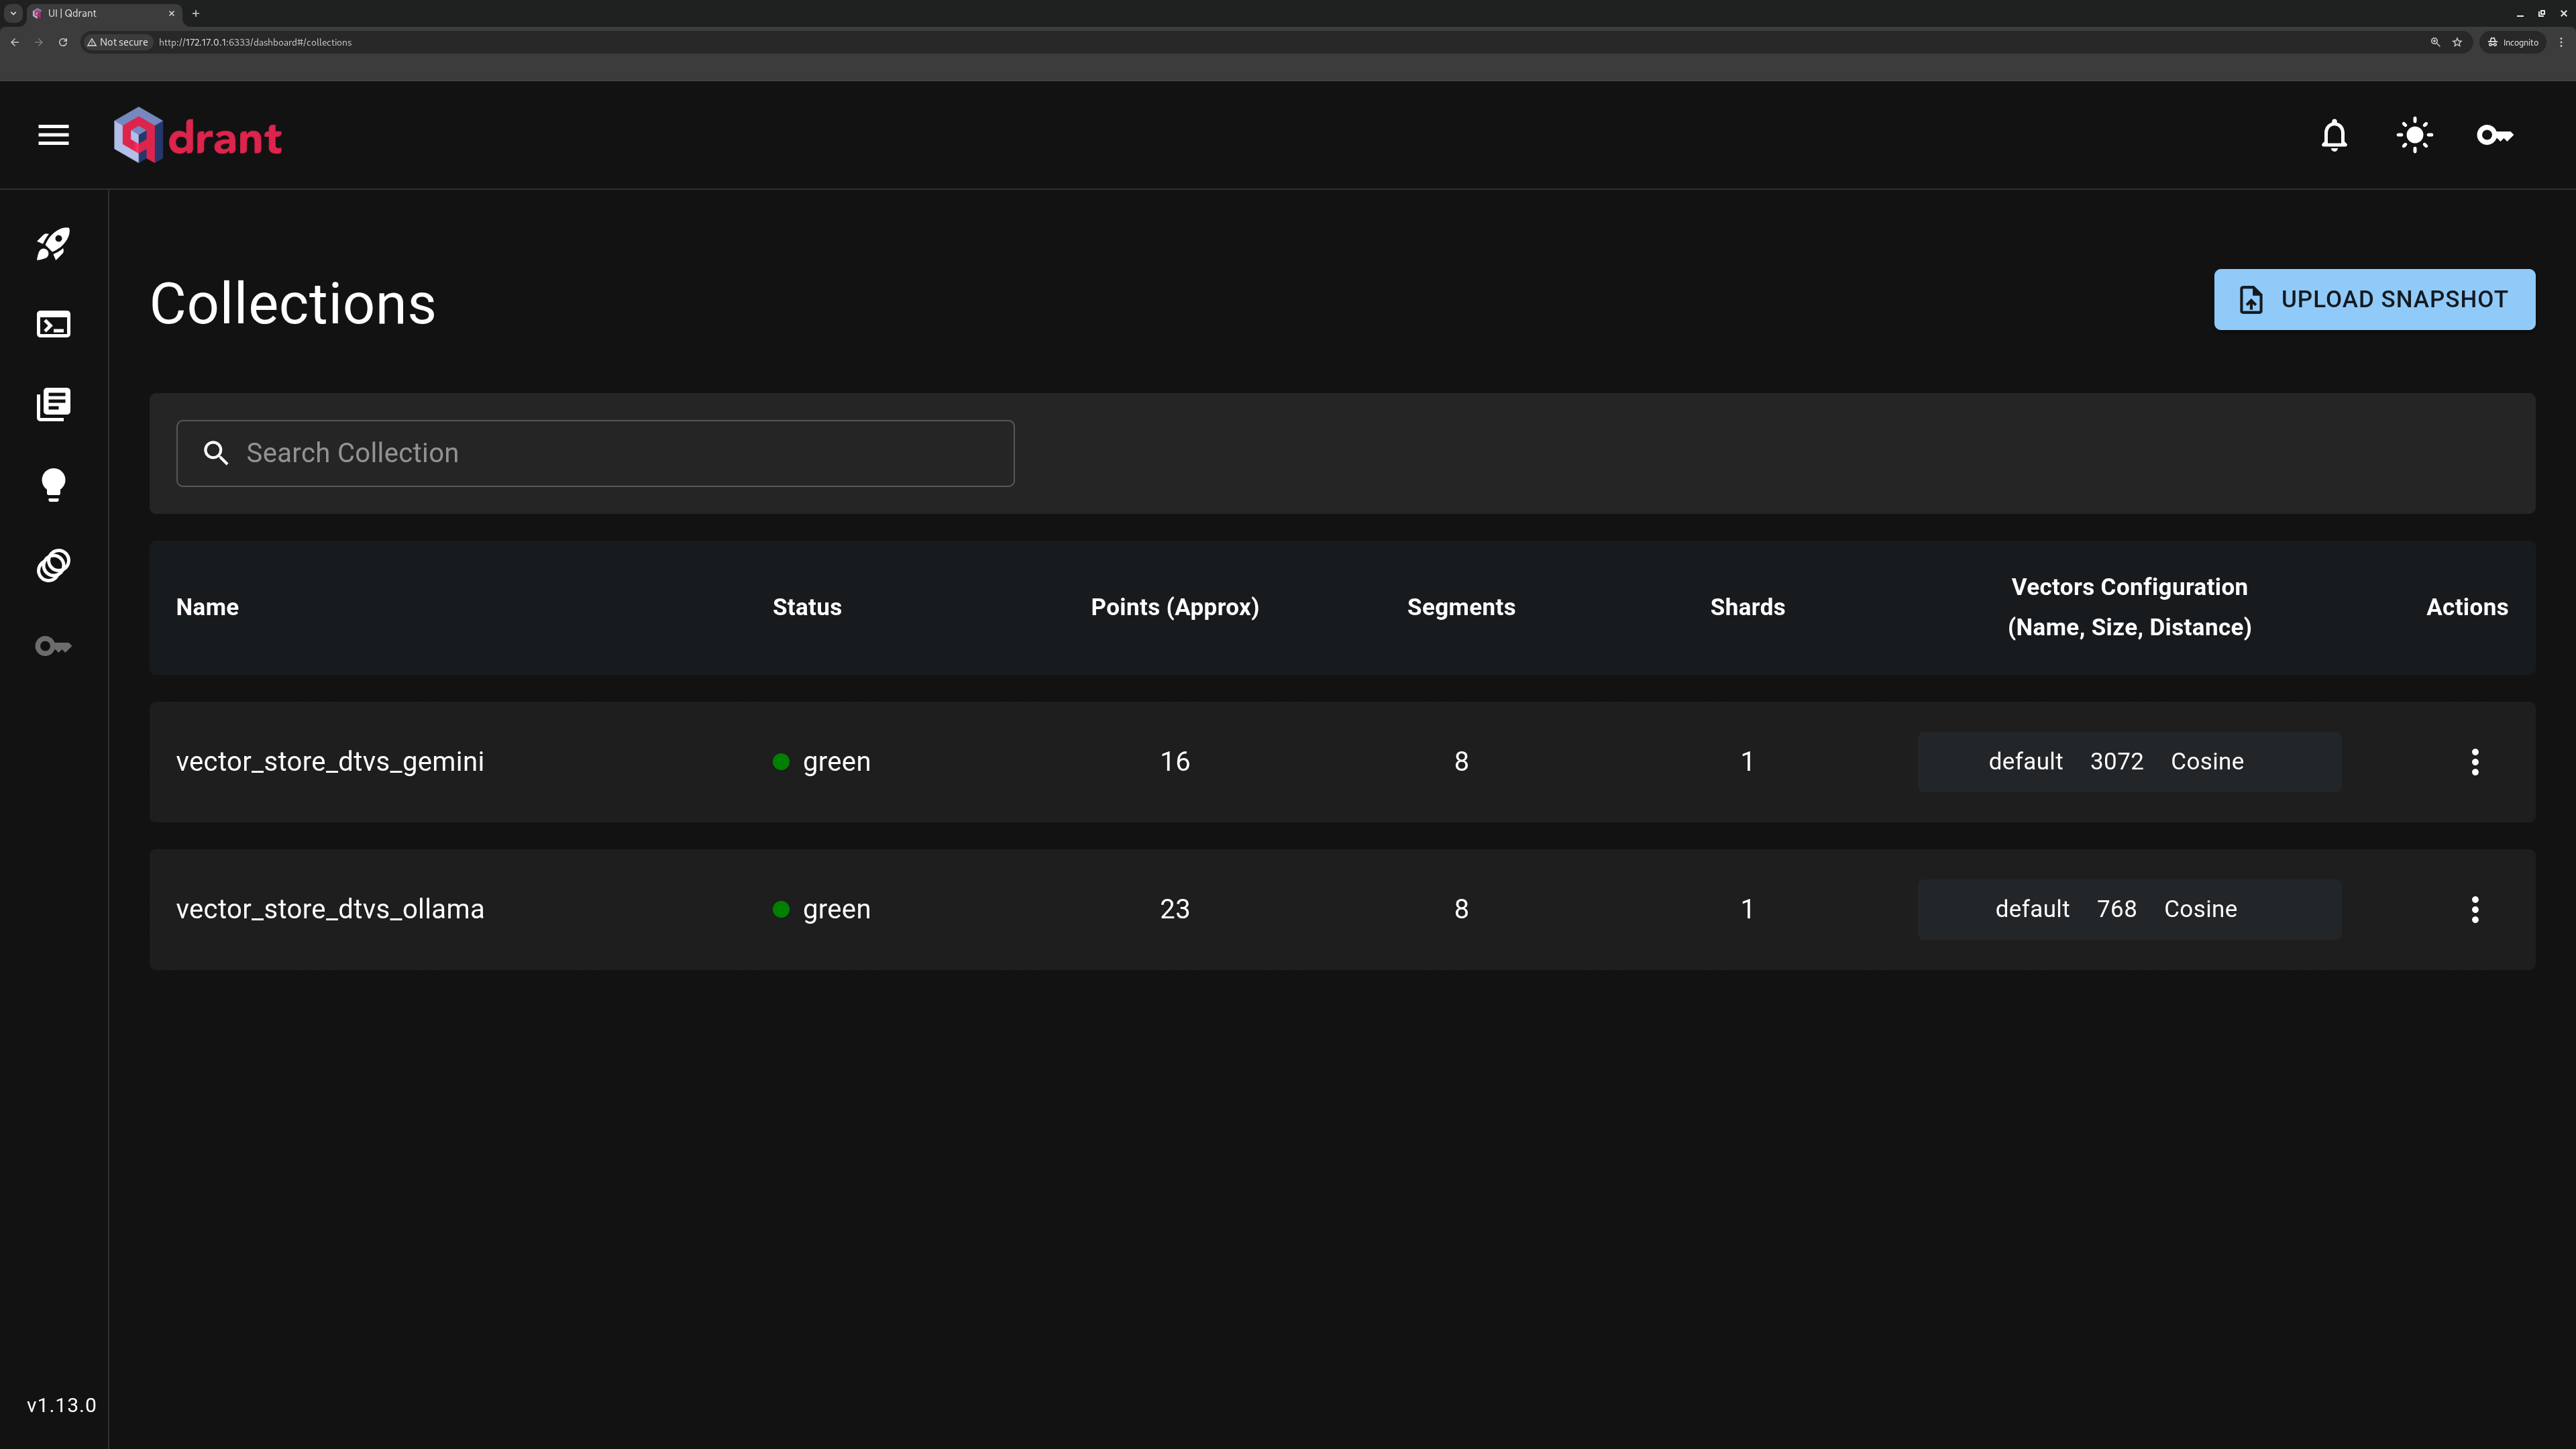
\includegraphics[width=\textwidth, frame]{img/qdrant-dashboard.png}
		    \end{figure}
	\end{minipage}
\end{frame}
%
\begin{frame}[fragile] \frametitle{Codice}
    \framesubtitle{Branch di riferimento}
	\begin{center}
		{\scriptsize \href{https://github.com/simonescannapieco/spring-ai-advanced-dgroove-venis-code.git}{\texttt{https://github.com/simonescannapieco/spring-ai-advanced-dgroove-venis-code.git}}}\\
		\textit{Branch:} \alert{\texttt{8-spring-ai-gemini-ollama-rag-document-to-vector-store}}
	\end{center}
\end{frame}